\documentclass[11pt]{article}
\usepackage{graphicx} %for displaying images
\usepackage{float}
\usepackage{listings}
\usepackage{color}

\definecolor{dkgreen}{rgb}{0,0.6,0}
\definecolor{gray}{rgb}{0.5,0.5,0.5}
\definecolor{mauve}{rgb}{0.58,0,0.82}

\lstset{frame=tb,
	language=Python,
	aboveskip=3mm,
	belowskip=3mm,
	showstringspaces=false,
	columns=flexible,
	basicstyle={\small\ttfamily},
	numbers=none,
	numberstyle=\tiny\color{gray},
	keywordstyle=\color{blue},
	commentstyle=\color{dkgreen},
	stringstyle=\color{mauve},
	breaklines=true,
	breakatwhitespace=true,
	tabsize=3
}

%----------------------------------------------------------------------------------------
%	TITLE SECTION
%----------------------------------------------------------------------------------------
\title{	
	\normalfont\normalsize
	\textsc{Old Dominion University}\\ % Your university, school and/or department name(s)
	\vspace{25pt} % Whitespace
	\rule{\linewidth}{0.5pt}\\ % Thin top horizontal rule
	\vspace{20pt} % Whitespace
	{\huge Assignment one}\\ % The assignment title
	\vspace{12pt} % Whitespace
	\rule{\linewidth}{2pt}\\ % Thick bottom horizontal rule
	\vspace{20pt} % Whitespace
}
\author{\LARGE Joshua Gahan} % Your name
\date{\normalsize\today} % Today's date (\today) or a custom date

\begin{document}
	\pagenumbering{gobble}
	\maketitle %render title
	\newpage
	\pagenumbering{arabic}
	
	\section{Tweet Collection }
	\hspace{10mm} Using the keyword 'Trump' we collected tweets via Twitter's Streaming API in order. to extract unique URIs. These URIs were output to a file "unparsedURLs.txt" for further processing. 
	
	\subsection{Retrieval of Tweets}
	\begin{lstlisting}
	class MyStreamListener(tweepy.StreamListener):
	    def __init__(self, num_tweets):
	        super().__init__()
	        self.num_tweets = int(num_tweets)
	        self.outFile = open("unparsedURLs.txt", 'a')
	        self.errFile = open("error_log", 'a')
	        self.foundURLs = 0  #used for output to console as a visual aid
	        self.parsedURLCount = 0 #used for output to console as a visual aid.
	        self.curious = 0
	    def on_status(self, status):
	        # regex to extract links from tweet
	        parsed_tweet = re.findall('https*:\/\/\S+', status.text)
	
	        self.curious += 1
	        for url in parsed_tweet:
	            self.outFile.write(url + '\n')
	            self.num_tweets -= 1
	            self.foundURLs += 1
	
	        if self.foundURLs % 20 == 0:
	           print("Found Urls: %d   Tweets Processed: %d" % (self.foundURLs, self.curious))
	
	        # False turns the stream off.
	        if self.num_tweets < 1:
	            return False
	
	    def on_error(self, status_code):
	        if status_code == 420:
	        #returning False in on_error disconnects the stream
	        return False
	\end{lstlisting}
	\hspace{10mm} MyStreamListener functions as the 'on data' listener for the tweepy.Stream object. When data is received, the on\_status function is called. We use a regex search to extract the URIs within a tweet and store them within parsed\_tweet. Finally we write the found URLs to unparsedURLS.txt. We utilize two variables: foundURLs and curious as helpers for giving meaningful output to the user as to the scripts current progress (printing our status out every 20 found URLs). Finally, we utilize a num\_tweets variable as a control variable. When a tweepy stream object receives "False", the stream is disabled. We utilize this behavior to allow us to operate the stream until a desired amount of links have been found (provided as a command line argument). 
	\begin{figure}[h!]
		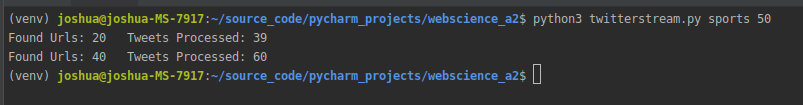
\includegraphics[scale=0.5]{resources/stream_console_out.png}
		\caption{Stream Console output}
	\end{figure}
	\begin{figure}[h!]
		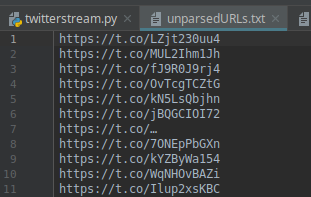
\includegraphics[scale=0.8]{resources/unparsedURLs.png}
		\caption{unparsedURLs.txt}
	\end{figure}
	\section{Extracted Link Processing. }
	\hspace{10mm} Utilizing multithreading we set ten threads to the task of resolving our extracted links to URLs. If these links are within the twitter domain they are discarded. Parsed URLs are then written to another intermediary file called "parsedURLs.txt" 
	\subsection{Link Processing}
	\begin{lstlisting}
	def processURL(thread_name, q, count):
	    while not exitFlag:
	        count += 1
	        queueLock.acquire()
	
	# follow the url until the location header isn't present, then check if its a twitter domain.
	# push onto threadsafe list, which will be fed into a set down the line to check for duplicates.
	    if not workQueue.empty():
	        url = q.get()
	        queueLock.release()
	        push = False
	        try:
	            res = requests.get(url)
	            url = res.url
	
	            while res.status_code == 301:
	                try:
	                    url = res.headers['location']
	                    res = requests.get(url)
	                except Exception as e:
	                    print("Error: ", str(e))
	
	            if url.find('twitter') < 0 and res.status_code == 200:
	                push = True
	            else:
	                push = False
	        except Exception as e:
	            print("some error " + str(e) + ": " + url)
	
	        if push == True:
	            notTwitter.append(url)
	    else:
	        queueLock.release()
	        time.sleep(1)
	
	    if len(notTwitter) % 25 == 0:
	        print("%d candidate links" % len(notTwitter))
	        
	        
	   # below is the file write which is not part of the above function. Note that goodURLs is a set. 
	   for item in notTwitter:
	       goodURLS.add(item + '\n')
	   with open("parsedURLs.txt", 'a') as outFile:
	       for entry in goodURLS:
	           outFile.write(entry)
	\end{lstlisting}
	\hspace{10mm} We start by pulling a url to test of the queue.  We then attempt a 'GET' call on the url. If the response contains status code 301 (a redirect) we then follow the redirect (this is done via a while loop that stops once it encounters a non-301 status code). Following this we do a string search of the parsed url, pushing any found urls that don't contain 'twitter' and result in a status code 200 ('OK') to notTwitter (a list). URLs that have been pushed to this notTwitter are then passed into a set "goodURLs" to utilize the properties of a set object for removing duplicates. this goodURL set is then wrote to an intermediary file "parsedURLs.txt".  
	
	\begin{figure}[h!]
		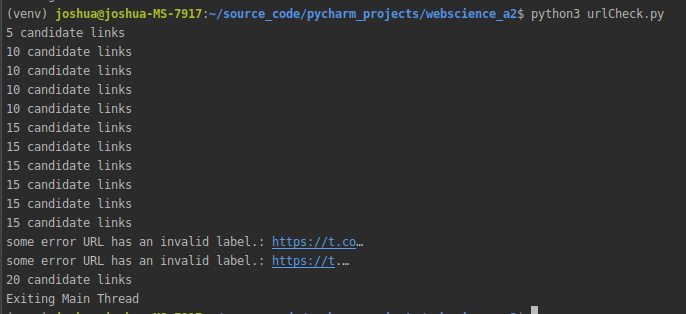
\includegraphics[scale=0.5]{resources/urlCheckConsole.png}
		\caption{URL Check output}
	\end{figure}
	\begin{figure}[h!]
		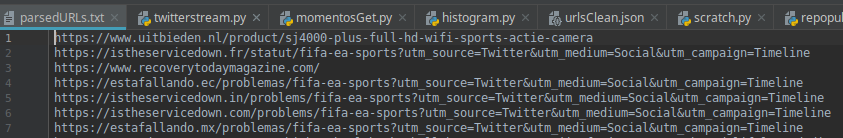
\includegraphics[scale=0.4]{resources/urlCheckOut.png}
		\caption{parsedURLs.txt}
	\end{figure}
	\section{Further Extracted Link Processing }
	\hspace{10mm} Having cleaned our data, we here push the URLs we wrote into 'parsedURLs.txt' to urlsClean.json file which will serve as our database for all further operations on the dataset. Below code simply reads in the parsed urls and instantiates the ursClean.json per our desired format (shown below). 
	\subsection{Further Link Processing}
	\begin{lstlisting}
	#initURL_json_db.py
	def initializeURLJSON():
	    # create backup of URL database file
	    backup = json.load(open("urlsClean.json"))
	    with open('urlsClean.bak', 'w') as json_file:
	        json.dump(backup, json_file)
	        json_file.close()
	
	    # reopen file and get count of URLS present. Store data in goodURL and count in goodURLCount
	    goodURL = json.load(open("urlsClean.json"))
	
	    with open('parsedURLs.txt', 'r') as urls:
	    for line in urls:
	        outUrl = line.strip()
	        goodURL["%s" % outUrl] = {"momentos": 0, "timeMapFilename": " ", "carbonDate": " "}
	
	    with open('urlsClean.json', 'w')as outFile:
	        pretty_data = json.dumps(goodURL, indent=4)
	        outFile.write(pretty_data)
	
	initializeURLJSON()
	\end{lstlisting}
	\begin{figure}[h!]
		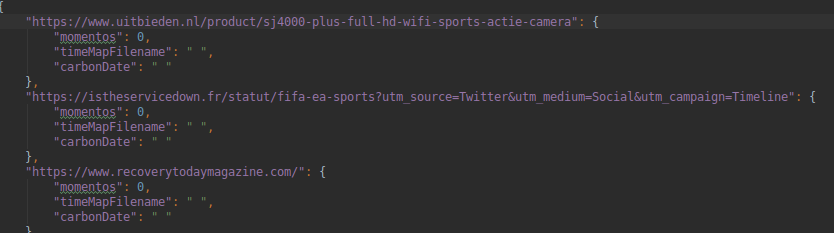
\includegraphics[scale=0.5]{resources/urlCleanFile.png}
		\caption{Example entries from urlsClean.json}
	\end{figure}
	\section{Further Extracted Link Processing }
		\hspace{10mm} Having finished collecting our data. We begin to process it in momentosGet.py. Here we read in our URL database and pass the URLs to Memgator to collect momento data. 
	\subsection{Memento Collection Algorithm }
	\begin{lstlisting}
	urls_to_Momentize = json.load(url_db)
	count = 0
	momento_count = 0
	for url in urls_to_Momentize:
	    if urls_to_Momentize[url]["momentos"] <= 0:
	        count += 1
	        try:
	            res = requests.get("%s/timemap/json/%s" % (memgator_url, url))
	            if(res.status_code == 200 or res.status_code == 302):
	                try:
	                    urls_to_Momentize[url]["momentos"] = res.headers['X-Memento-Count']
	                    momento_count += int(res.headers['X-Memento-Count'])
	                    if urls_to_Momentize[url]["timeMapFilename"] == " ":
	                        timeMapFileName = "%d.txt" % abs(hash(url))
	                    else:
	                        timeMapFileName = urls_to_Momentize[url]["timeMapFilename"]
 	                    with open("./timemaps/%s" % timeMapFileName, 'w') as outFile:
	                        outFile.write(res.text)
	                    urls_to_Momentize[url]["timeMapFilename"] = timeMapFileName
	                except Exception as e:
	       print("Error: ", str(e))
	\end{lstlisting}
	\hspace{10mm} After loading our urls from urlsClean.json we check for each URL if mementos have already been populated, if not we make a request to the provided Memgator URL. If Memgator returns either a 200 or 302, we extract the Memento count from the 'X-Memento-Count' header.  We then create (or open if it exists) a text file  containing the json output of the response (if status code 300 or 302) which is named based on the hash of the url. Finally. We take the name of this file we have just created and add it to our database for easy indexing later. 
	\subsection{Memgator Processing}
	\begin{figure}[h!]
		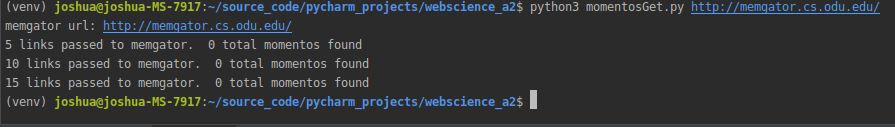
\includegraphics[scale=0.5]{resources/memgator_console.png}
		\caption{console log of using memgator}
	\end{figure}
	\begin{figure}[h!]
		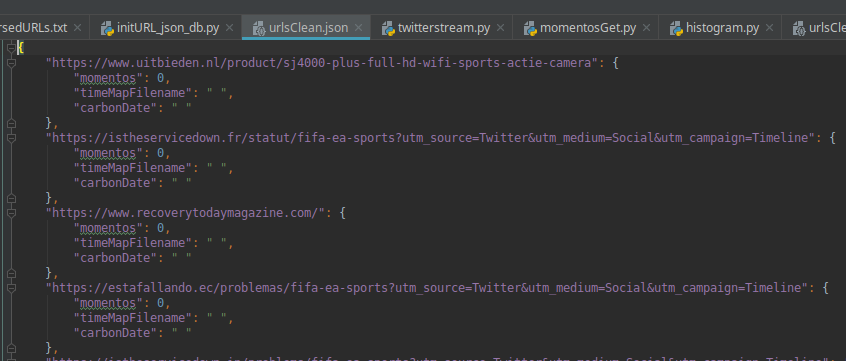
\includegraphics[scale=0.5]{resources/memgator_out.png}
		\caption{our updated JSON. Note: for demo purpose, we are working with a limited dataset, hence no mementos.}
	\end{figure}
	\section{CarbonDate }
	\hspace{10mm} Utilizing the same urlsClean.json database, we then use the CarbonDate service to estimate the creation date of the URLS within urlsClean.json .
	\subsection{CarbonDate Algorithm }
	\begin{lstlisting}
	def processURL(thread_name):
	    while not exitFlag:
	        global count
	        global workQueue
	        global goodURL
	        count += 1
	        queueLock.acquire()
	
	        if not workQueue.empty():
	           url = workQueue.get()
	           queueLock.release()
	           try:
	               res = requests.get("%s/cd/%s" % (carbondate_url, url))
	               responseJSON = json.loads(res.text)
	               creationDate = responseJSON["estimated-creation-date"]
	               goodURL[url]["carbonDate"] = creationDate
	           except Exception as e:
	               print("Error: ", str(e))
	
	           if count % 25 == 0:
	              print("%d links passed to carbondate. Executed by thread: %s" % (count, thread_name))
	\end{lstlisting}
	\hspace{10mm} Utilizing the same multithreaded scheme used before, each thread pulls urls from a queue and executes the function above. We make a request to the carbondate service and store the response JSON in responseJSON. Within this responeJSON we extract the value from the "estimated-creation-date" key. we then push this found date to our JSON database (urls are used as keys for urlsClean.json) 
	\begin{figure}[h!]
		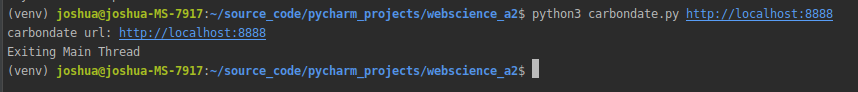
\includegraphics[scale=0.5]{resources/carbon_console.png}
		\caption{console log of using carbondate.py}
	\subsection{Carbondate processing}
	\end{figure}
	\begin{figure}[h!]
		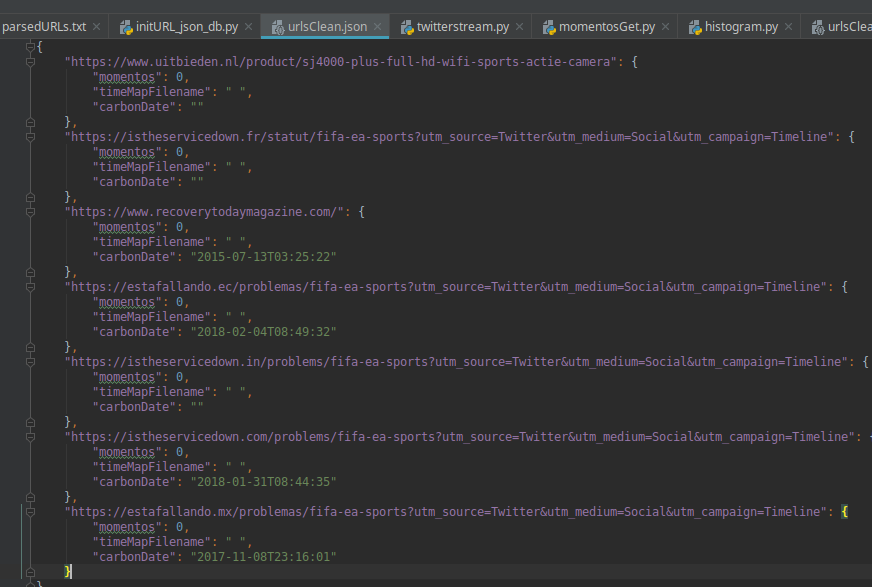
\includegraphics[scale=0.5]{resources/carbon_out.png}
		\caption{our updated JSON following carbondating}
	\end{figure}
	\section{Findings}
	\hspace{10mm}We found by that the overwhelming majority of URLs did not possess memento representations. This could be that we used "Trump" as our keyword and thus the vast majority of our URLs linked to recent news and events. As the number of mementos increased, the number of URLs possessing that many mementos decreased. We had some outliers, such as URLs with over 50,000 mementos, but just over 76\% of our URLs had between 0 and 2 mementos. 
	\begin{figure}[h!]
		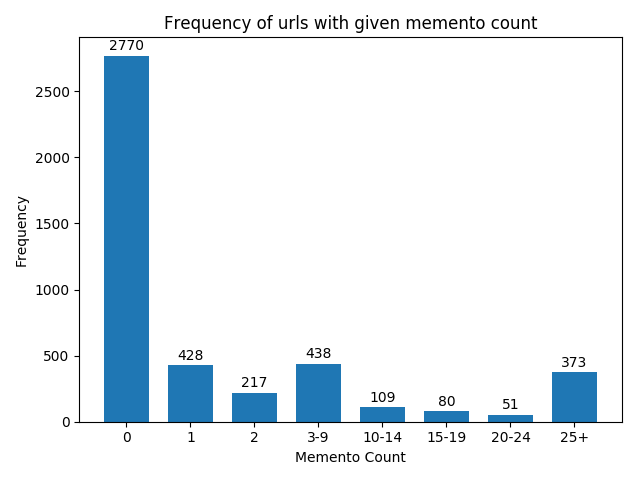
\includegraphics[scale=0.6]{resources/memento_count__vs__URI_count.png}
		\caption{\#of urls possessing x number of mementos}
	\end{figure}
	\hspace{10mm} In looking at estimated CarbonDate reported date vs memento count, one would hypothesize that as the age of a site increases, so to would the number of mementos for that sight in a more or less linear fashion. The graph below shows our findings (Note that URLs with memento counts greater than 50,000 have been excluded as data points below).  
	\begin{figure}[h!]
		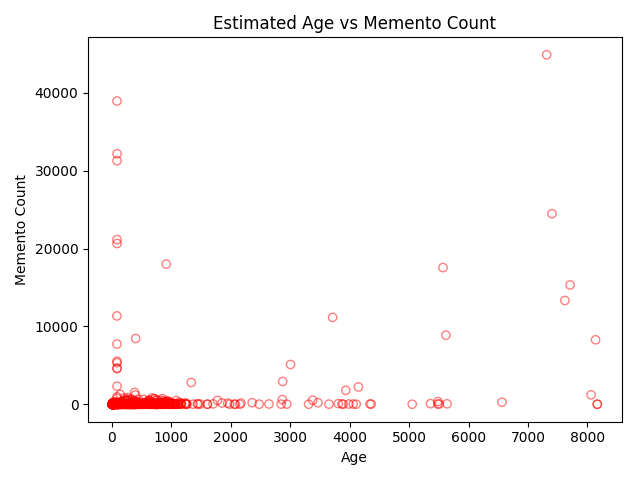
\includegraphics[scale=0.6]{resources/scatter_50k.png}
		\caption{Estimated age of site vs Memento Count}
	\end{figure}
	\subsection{Suspicion of Data}
	\hspace{10mm} We find ourselves suspicious of these data points however. The carbondate was only set when we received a date from the Carbondate server, and was not set otherwise, but it is the suspicion of the author that that we encountered throttling and CarbonDate was filling in the date with the current date. The graph attached as an appendix after the conclusion we believe shows this. 
	\begin{figure}[h!]
		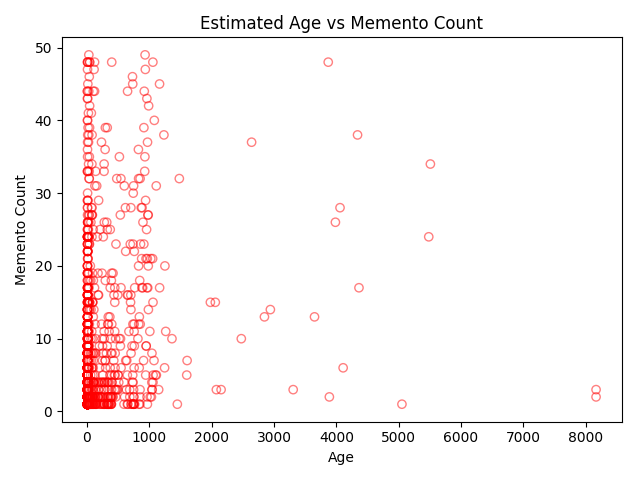
\includegraphics[scale=0.6]{resources/carbondate50.png}
		\caption{Estimated age of site vs Memento Count}
	\end{figure}
	\section{Conclusion}
		Despite our suspicions of the CarbonDate vs Memento count data, our collected data lines up well with the hypothesis that there is a linear relationship between the age of a site and the number of times it has been archived. A further investigation of the reported creation dates, might tease out if the data is incorrect due to the above hypothesis, correct but aberrant data, or if our hypothesis is incorrect. 
	  
	
	
	
	
	
\end{document}